\documentclass{standalone}
\usepackage{tikz,amsmath,graphicx,calc,chemfig}
\usepackage[update,verbose=false]{epstopdf}
\usepackage[version=3]{mhchem}
\graphicspath{{./figs/}}
\usetikzlibrary{
    arrows,
    decorations.pathmorphing,
    backgrounds,
    positioning,
    fit,
    petri
}
\setatomsep{1.4em}
\setbondoffset{.1em}
\setcrambond{.3em}{1pt}{.1em}
%\setbondstyle{thick}
\renewcommand*\printatom[1]{{\footnotesize\ensuremath{\mathsf{#1}}}}


\begin{document}
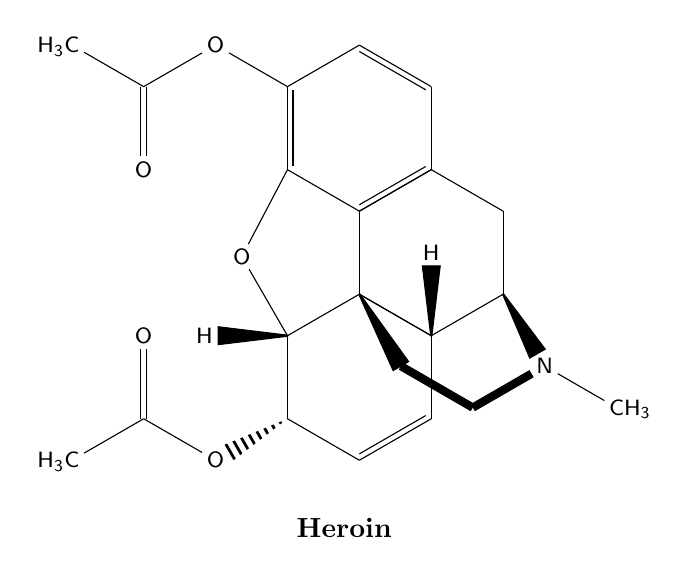
\begin{tikzpicture}
    [scale=1,
     structure/.style={rectangle,draw=white,fill=white,
               outer xsep=.2cm,outer ysep=.2cm,minimum size=2mm,node distance=1.4cm},
     label/.style={rectangle,fill=white,font=\bfseries,
               outer ysep=.2cm,minimum size=4mm,},
     arrow/.style={->,>=stealth',semithick},
     reagent/.style={text width=2cm,font=\footnotesize,align=center,midway},
     designbox/.style={rectangle,draw=black,thick,fill=red,
               inner sep=0pt,minimum width=15mm, minimum height=2.5mm, node distance=0mm}]
    %
    \node[structure] (Heroin) {\chemfig{
        [:30]H_3C-(=[::60]O)-[::-60]O>:*6(-=-*6(-?[2]--*6(-=-(-O-[::60](-[::-60]H_3C)=[::60]O)=?[1]-=)---)(<[::0]H)-(<[::150]-[::30,,,,line width=.3em]-[::60,,,,line width=.3em]N?[2,{<}](-[::-60]CH_3))-(<[::-30]H)(-[::-90,1.1]O?[1])-)
    }};

    \draw (Heroin.south)      node[label,yshift=-0.4cm]{Heroin};
\end{tikzpicture}
\end{document}
